\documentclass[11pt]{article}
\usepackage{theme}
\usepackage{shortcuts}
\usepackage{algorithm}
\usepackage[noend]{algpseudocode}
\usepackage{mathtools}
\usepackage{amsmath}
\usepackage{stmaryrd}
\usepackage[numbers,square]{natbib}
% Document parameters
% Document title 
\title{Detecting Changes in Slope With an $L_0$ Penalty}
\author{
Bastien LE CHENADEC \email{bastien.le-chenadec@eleves.enpc.fr} \\ % student 1
Sofiane EZZEHI \email{sofiane.ezzehi@eleves.enpc.fr} % student 2
}

\begin{document}
\maketitle
\section{Introduction and contributions}

Changepoints detection is an important problem in time series analysis. It consists in finding the points in time where the statistical properties of the signal change. The problem can be modeled as a parametric approximation of the original signal to which a cost function is associated \cite{Truong_Oudre_Vayatis_2020}. Finding the approximation with minimal cost is generally a dynamic programming problem. In \cite{main_article}, the authors propose a piecewise continuous model for the signal, penalized by an $L_0$ penalty on the number of changepoints.

\paragraph*{Contributions}
While an implementation of the algorithm was already available online in R and C++, we chose to implement it ourselves from scratch in Python.

Both contributors spent a considerable amount of time on the implementation of the algorithm. While, Bastien L.C. implemented the algorithm in Python and heavily optimized it to make it run in a reasonable time, Sofiane E. thoroughly debugged the algorithm (notably finding and correcting errors in the original paper's computations), and ran the experiments. The report was jointly written by both contributors.

 We chose to test the algorithm on Tunisian stock market data, and we experimented with different values of the penalty parameter $\beta$ and the segment cost $h$.

\section{Method}

Let $y=y_1, \dots, y_n$\footnote{A word on notations : if we have a sequence $x=x_1,\dots,x_n$, we denote $x[s:t]$ the subsequence $x_s,\dots,x_t$.} $\in \mathbb{R}^n$ be successive data points in time. We aim to find $m$ changepoints $\tau_1,\dots,\tau_m$ such that the data is divided in $m+1$ segments. We let $\tau_0=0$ and $\tau_{m+1}=n$; the segment $j$ is then $y_{\tau_{j-1}+1},\dots,y_{\tau_j}$. The number of changepoints $m$ is assumed unknown.

\subsection{Model}

The parametric model considered is a continuous piecewise linear model. We denote $\phi_{\tau_j}$ the value taken by the model at time $\tau_j$. Under these assumptions, the model writes :
\begin{equation}
    \forall i\in \llbracket0,m\rrbracket,\,\forall t \in \llbracket\tau_i+1,\tau_{i+1}\rrbracket, \quad Y_t=\phi_{\tau_i}+\frac{\phi_{\tau_{i+1}}-\phi_{\tau_i}}{\tau_{i+1}-\tau_i}(t-\tau_i)+Z_t
\end{equation}
where $(Z_t)_{1\leq t\leq n}$ is assumed to be a gaussian white noise with variance $\sigma^2$.

\subsection{Penalized cost approach}

In order to find the parameters $m, \tau_1,\dots,\tau_{m}, \phi_{\tau_0},\dots, \phi_{\tau_{m+1}}$, we adopt a penalized cost approach. The cost function is a squarred error loss, penalized by a term that depends on the segments length, and an $L_0$ penalty on the number of changepoints. The cost function writes :
\begin{equation}
    \sum_{i=0}^m \left[\frac{1}{\sigma^2}\sum_{t=\tau_i+1}^{\tau_{i+1}} \left(y_t-\phi_{\tau_i}-\frac{\phi_{\tau_{i+1}}-\phi_{\tau_i}}{\tau_{i+1}-\tau_i}(t-\tau_i)\right)^2 + h(\tau_{i+1}-\tau_i)\right]+\beta m
\end{equation}
To simplify the notations we introduce the cost function for fitting a segment that takes the value $\phi$ at time $s$ and $\psi$ at time $t$ :
\begin{equation}
    \mathcal{C}(y[s+1:t],\phi,\psi) = \frac{1}{\sigma^2}\sum_{j=s+1}^t \left(y_j-\phi-\frac{\psi-\phi}{t-s}(j-s)\right)^2
\end{equation}
The optimisation problem then writes :
\begin{equation}
    \label{eq:problem}
    \min_{\substack{m\\\tau_1,\dots,\tau_m\\ \phi_0,\dots,\phi_{m+1}}} \sum_{i=0}^m \left[\mathcal{C}(y[\tau_i+1:\tau_{i+1}],\phi_{\tau_i},\phi_{\tau_{i+1}}) + h(\tau_{i+1}-\tau_i)\right] + \beta m
\end{equation}

\subsection{Dynamic programming}

Problem \eqref{eq:problem} can be solved by dynamic programming. Compared to other changepoints detection methods, the difficulty lies in the continuity constraint between segments. Let $f^t(\phi)$ be the minimum cost for segmenting $y_1,\dots,y_t$ conditionally on the model taking the value $\phi$ at time $t$ :
\begin{equation}
    \begin{aligned}
        f^t(\phi)=\min_{\substack{k                                             \\\tau_1,\dots,\tau_{k}                         \\ \phi_0,\dots,\phi_k}} &\sum_{i=0}^{k-1} \left[\mathcal{C}(y[\tau_i+1:\tau_{i+1}],\phi_{\tau_i},\phi_{\tau_{i+1}}) + h(\tau_{i+1}-\tau_i)\right]\\
         & +\mathcal{C}(y[\tau_k+1:t],\phi_{\tau_k},\phi)+h(t-\tau_k) + \beta k
    \end{aligned}
\end{equation}
$f^t(\phi)$ can be expressed recursively :
\begin{equation}
    f^t(\phi)=\min_{\phi',s} f^s(\phi')+\mathcal{C}(y[s+1:t],\phi',\phi)+h(t-s)+\beta
\end{equation}
To handle the cost of a specific segmentation let $f^t_{\boldsymbol{\tau}}(\phi)$ be the minimum cost for segmenting $y_1,\dots,y_t$ conditionally on the model taking the value $\phi$ at time $t$ and the changepoints being $\boldsymbol{\tau}=(\tau_0,\tau_1,\dots,\tau_k)$. $f^t_{\boldsymbol{\tau}}$ is a quadratic polynomial in $\phi$ and its coefficients can be expressed recursively. The coefficients given in Appendix C of the supplementary material of \cite{main_article} are not correct. We provide the correct coefficients in the Appendix \ref{appendix:coefficients}.

\subsection{Pruning}

Given the exponential complexity of the dynamic programming algorithm ($\mathcal{O}(2^n)$ possible segmentations), the authors introduce two pruning techniques to reduce it.

\subsubsection{Functional pruning} Let $\mathcal{T}_t$ be the set of all possible changepoint vectors for segmenting $y_1,\dots,y_t$, and $\mathcal{T}_t^*=\left\{\boldsymbol{\tau}\in \mathcal{T}_t \:\big|\: \exists\phi\in\mathbb{R}, f^t(\phi)=f_{\boldsymbol{\tau}}^t(\phi)\right\}$ the set of changepoint vectors at time $t$ that are optimal for some $\phi$. The following result reduces the number of segmentations to consider at time $t+1$.

\begin{theorem}
    \label{th:functional_pruning}
    Let $\boldsymbol{\tau}\in\mathcal{T}_s$ such that $\boldsymbol{\tau}\notin \mathcal{T}_s^*$. Then $\boldsymbol{\tau}\notin \mathcal{T}_t^*$ for all $t>s$.
\end{theorem}

\subsubsection{Inequality based pruning} Let $K=2\beta+h(1)+h(n)$. Suppose that $h$ is non-negative and non-decreasing. The following result reduces the number of segmentations to consider at time $t+1$.

\begin{theorem}
    Let $\boldsymbol{\tau}\in\mathcal{T}_s$ such that :
    $$\min_\phi f_{\boldsymbol{\tau}}^s(\phi) > K + \min_{\phi'} f^s(\phi')$$
    Then $\boldsymbol{\tau}\notin \mathcal{T}_t^*$ for all $t>s$.
\end{theorem}

This theorem allows to further prune the set $\hat{\mathcal{T}}_t$.

\subsection{Algorithm}

The algorithm consists in computing the coefficients of the polynomials $f^t_{\boldsymbol{\tau}}(\phi)$ iteratively, starting from $f^0(\phi)$. At each step, the set of possible segmentations is pruned using the two pruning techniques. The algorithm is detailed in appendix \ref{appendix:algorithms}.

The main difficulty of this algorithm is that we need to store polynomial coefficients instead of cost values. We also have to be careful to store only the coefficients that will be needed in recursive calls ($f^{\tau_k}_{\tau_1,\dots,\tau_{k-1}}$) to avoid memory issues. Overall avoiding re-allocating memory at each step was a challenge to implement the algorithm efficiently.

The authors provided relatively detailed pseudo-code for the algorithm, but we still found it difficult to implement. One difficulty was that the coefficients updates given in the paper were not correct, which took a lot of time to figure out.

\section{Data}
\subsection{Data description : Tunisian stock market}
Financial data, and more specifically stock prices across time, are a good candidate to test the method. Indeed, stock prices, taken at a relatively low frequency (daily) are known to exhibit clear trends, while being noisy enough to make the detection of changepoints interesting. And since the method is designed to detect changepoints in a piecewise linear model, it is well suited for this kind of data.

We test the method on the stock prices of all the listed companies on the Bourse de Tunis, which is Tunisia stock exchange. The data was taken from Kagglee, and is available at \url{https://www.kaggle.com/datasets/amariaziz/tunisian-stock-market}. It contains the Open, High, Low and Close prices of 88 companies, as well as the volume of transactions. We only use the Close prices, which are the prices at the end of the trading day.
\subsection{Data preprocessing}
Since the data was partially collected by web scraping, it naturally requires some cleaning and preprocessing. We detail here the steps we took to clean the data.
\paragraph*{Stocks with too few data points} We see on figure \ref{fig:histogram_size} that the number of data points per company is very variable. We remove the stocks that have less than $200$ data points, since they are not interesting for our analysis. We are left with $85$ companies.
\paragraph*{Missing values and duplicates} Missing values are days where we have corrupted data for a given stock. We see in table \ref{tab:missing_values} that the data is relatively clean of missing values, with only $3$ companies having no more than a few percent of corrupted data. We see on figure \ref{fig:bar_duplicates} that each stock has between $1\%$ and $3\%$ of duplicates. We remove the missing values as well as the duplicates.
\paragraph*{Missing days} Missing days are days where we have no data at all for a given stock. We see on figure \ref{fig:bar_missing_days} that the number of missing days is clearly the biggest issue with the data, with most stocks having more than $40\%$ of missing days. We deal with this issue by linearl interpolating the missing days between the last and next available data points. We note that this is not a perfect solution, since it assumes that the stock price evolves linearly between two days. However, it is a simple solution that allows us to keep the data for all the stocks.
\paragraph*{Data shrinkage by sub-sampling} Since our method is relatively slow for time series longer than a few thousand points, and since our available computational power is limited, we uniformly sub-sample the data to reduce its size, only keeping at most $500$ points per stock. We see on figure \ref{fig:subsample} that this sub-sampling very slightly affects the shape of the signal.

\section{Results}
We present here a few experiments that we conducted on the $85$ Tunisian stocks we preprocessed. First, we zoom on a particular stock to see how the method behaves and we qualitatively compare it to a best-fitting piecewise constant mean model. Second, we investigate the influence of the penalty parameter $\beta$ on the number of changepoints detected. Third, we investigate the influence of the segment cost $h$ on the number of changepoints detected.

In all the experiments, we use a segment cost $h$ of the form $ h(s) = \gamma \log(s), $ where $\gamma$ is a parameter to fix and $s$ is the length of the segment. We also fix the parameter $\sigma$ depending on the stock, by using the very classical Median Absolute Deviation (MAD) estimator first introduced in \cite{hampel1974}.
\subsection{Qualitative comparison with a piecewise constant mean model}
We compare the method to a piecewise constant mean model, which is the simplest model that can be used to detect changepoints. We note that the nature of the data (stock prices) puts the piecewise constant mean model at a great disadvantage, since stock prices are known to exhibit piecewise linear trends. We only perform this comparison qualitatively.
\begin{figure}[h]
    \centering
    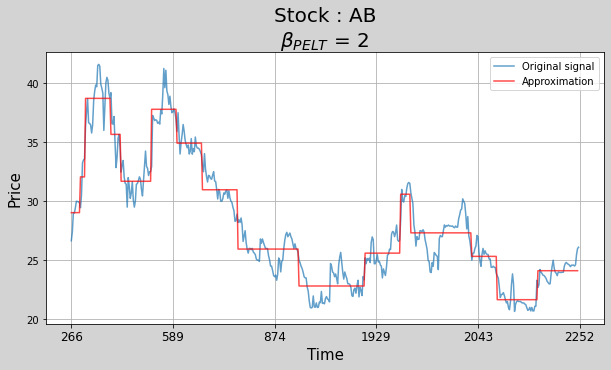
\includegraphics[width=0.495\textwidth]{figures/comparaison CPOP PELT/PELT.png}
    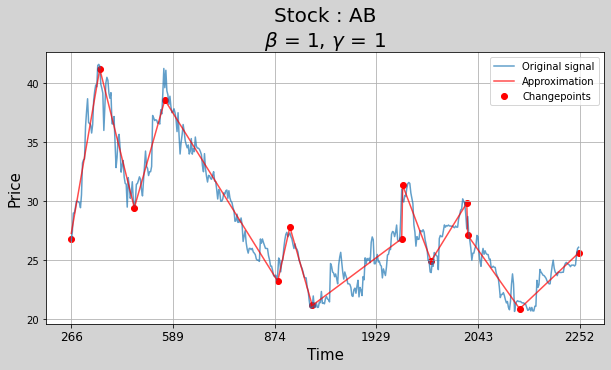
\includegraphics[width=0.495\textwidth]{figures/comparaison CPOP PELT/CPOP.png}
    \caption{Comparison of the PELT method (left) and the CPOP method (right) on the stock of the company "Amen Bank" (AB).}
    \label{fig:comparison}
\end{figure}

We see on figure \ref{fig:comparison} that the CPOP method is able to detect the changepoints much more accurately than the PELT method. More precisely, the PELT method exhibits a clear tendency to detect multiple changepoints between two consecutive CPOP changepoints. This is due to the fact that the PELT method is, by design, only able to detect changes in the mean of the signal; Therefore, along a steep trend, as the signal rapidly and monotonically varies, it will detect multiple changepoints, while the CPOP method will only detect one changepoint at the beginning of the trend and one at the end.

\subsection{Influence of the penalty parameter $\beta$}
Next, we investigate the influence of the penalty parameter $\beta$ on the number of changepoints detected. We see on figure \ref{fig:cgpts_beta} that the number of changepoints is a decreasing function of $\beta$, which is natural since $\beta$ penalizes the number of changepoints. We visualize the approximations obtained for values of $\beta \in \{0.1, 1, 5, 10, 20\}$ and $\gamma = 1$, on figure \ref{fig:approximations_beta}.

In particular, on figure \ref{fig:approximations_beta}, we see that almost all the data points are being detected for $\beta=0.1$ which, again, is a very normal behaviour, since we get a very minimal mean-square error $\sum C$ as well as a very small cost for the segments $\sum h$ if we allow for a lot of changepoints.

Furthermore, we see that the number of changepoints detected is the same for $\beta = 10$ and $\beta = 20$. This is due to the fact that the segment length cost $\sum h$, as well as the mean-square error $\sum C$ are both dominant compared to the effect of $\beta$, for values in this $[10,20]$ range.

\subsection{Influence of the segment cost $h$}
We used the same methodology to investigate the influence of the segment cost $h$ on the number of changepoints detected. We recall that the segment cost $h$, which penalizes the length of the segments, was chosen of the form,
$$ h(s) = \gamma \log(s), $$ where $\gamma$ is the parameter we will vary in this experiment.

We see on figure \ref{fig:approximations_gamma} the influence of $\gamma$ on the predicted approximation. An interesting phenomenon is that we could at first expect that, in order to reduce $h$, the algorithm would tend to split the largest segments into smaller segments, but we see that this is not the case. Indeed, since the segment cost is logarithmic, the algorithm tends to split the smallest segments into even smaller segments, which is why we see that the number of changepoints detected doesn't necessarily decrease when $\gamma$ increases. Furthermore, this explains why, as $\gamma$ increases, we see distinct parts of the signal with a denser number of changepoints.


\bibliography{bibliography}

\newpage
\section{Appendix}

\subsection{Algorithms}
\label{appendix:algorithms}
This algorithm keeps the polynomials that are optimal on some part of the real curve, by starting at $-\infty$ and iteratively finding the next optimal polynomial.
\begin{algorithm}[H]
    \caption{Functional pruning algorithm}
    \begin{algorithmic}[1]
        \State \textbf{Input:} Candidate segmentations $\hat{\mathcal{T}}_{t}$, costs $f^{t}_{{\tau}}(\phi)$ for ${\tau}\in\hat{\mathcal{T}}_{t}$.

        \State \textbf{Initialize:} $\phi_\text{curr}=-\infty \quad {\tau}_{curr}=\underset{{\tau}\in\hat{\mathcal{T}}_{t}}{ \arg\min}\left[f^{t}_{{\tau}}(\phi_{curr})\right]\quad \mathcal{T}_{temp}=\hat{\mathcal{T}}_{t}\setminus \left\{\tau_{curr}\right\}\quad \mathcal{T}^*_t=\left\{\tau_{curr}\right\}$

        \While{$\mathcal{T}_{temp}\neq\emptyset$}

        \For{$\tau\in\mathcal{T}_{temp}$}
        \State $x_{\tau}=\min\left\{\phi:f^{t}_{\tau}(\phi)-f^{t}_{{\tau}_{curr}}(\phi)=0\;\;\&\;\;\phi>\phi_{curr}\right\}$
        \If {$x_{\tau}=\emptyset$}
        \State $\mathcal{T}_{temp}=\mathcal{T}_{temp}\setminus\left\{\tau\right\}$
        \EndIf
        \EndFor

        \State $\mathcal{T}_{temp}=\mathcal{T}_{temp}\setminus \left\{\tau_{curr}\right\}$
        \State $\tau_{curr}=\underset{\tau\in\mathcal{T}_{temp}}{\arg\min}(x_{\tau})$
        \State $\phi_{curr}=x_{\tau_{curr}}$
        \State $\mathcal{T}^*_t=\mathcal{T}^*_t\cup\left\{\tau_{curr}\right\}$
        \EndWhile

        \State \textbf{Output:} $\mathcal{T}^*_t$
    \end{algorithmic}
\end{algorithm}
This algorithm is the main algorithm, it computes the coefficients of the polynomials and prunes the set of segmentations. The coefficients updates are detailed the appendix.
\begin{algorithm}[H]
    \caption{CPOP}
    \begin{algorithmic}[1]
        \State \textbf{Input:} Data $y=y_1,\dots,y_n$, penalty $\beta$ and segment cost $h$.

        \State \textbf{Initialize:} $\hat{\mathcal{T}}_1=\left\{\left\{0\right\}\right\}$

        \For {$t=1,\dots,n$} \Comment{Cost computation}
        \For {$\tau\in\hat{\mathcal{T}}_t$}
        \If {$\tau = \left\{0\right\}$}\Comment{No changepoint}
        \State $f^t_{\tau}(\phi)=\min_{\phi'}\mathcal{C}(y[1:t],\phi',\phi)+h(t)$
        \Else \Comment{Compute recursively}
        \State $f^t_{\tau}(\phi)=\min_{\phi'}\left(f^{\tau_k}_{\tau_1,\dots,\tau_{k-1}}(\phi')+\mathcal{C}(y[\tau_k+1:t],\phi',\phi)+h(t-\tau_k)+\beta\right)$
        \EndIf
        \EndFor

        \State $\mathcal{T}^*_t = \text{functional\_pruning}(\hat{\mathcal{T}}_t, f^t)$

        \State $\hat{\mathcal{T}}_{t+1}= \left\{\tau\in \hat{\mathcal{T}}_t \big| \min_\phi f_\tau^t(\phi)\leq \min_{\phi',\tau'}f_{\tau'}^t(\phi')+K\right\}\cup \left\{(\tau, t)\big|\tau\in \mathcal{T}^*_t\right\}$
        \EndFor

        \State \textbf{Output:} $\argmin_{\tau\in \hat{\mathcal{T}}_n}[\min_\phi f^n_\tau(\phi)]$
    \end{algorithmic}
\end{algorithm}
\clearpage
\subsection{Correction of the computed coefficients of the polynomials $f^t_{\boldsymbol{\tau}}(\phi)$}
\label{appendix:coefficients}
The authors provide a calculation of the coefficients of the polynomials $f^t_{\boldsymbol{\tau}}(\phi)$ in Appendix C of the supplementary material of \cite{main_article}. However, we found several mistakes in their calculations. We detail here the corrections we made.

The computation of the coefficients $A,\dots,F$ of $\mathcal{C}(y_{\tau_k+1:t},\phi',\phi)$ is correct. We therefore take,
\begin{equation}
    \mathcal{C}(y_{\tau_k+1:t},\phi',\phi) = A\phi^2+B\phi'\phi + C\phi + D + E\phi'+F{\phi'}^2,
\end{equation}
with the coefficients $A,\dots,F$ given by the authors.

We have to solve the following minimization problem,
\begin{equation}
    f_{\boldsymbol{\tau}}^t(\phi) = \min_{\phi'}\underbrace{\left(f^{\tau_k}_{\tau_1,\dots,\tau_{k-1}}(\phi')+\mathcal{C}(y_{\tau_k+1:t},\phi',\phi)+h(t-\tau_k)+\beta\right)}_{\vcentcolon = g_\phi(\phi')}.
\end{equation}
We note that $g_\phi$ is a quadratic polynomial in $\phi'$ since $\mathcal{C}$ is a quadratic polynomial in $\phi'$ and $f^{\tau_k}_{\tau_1,\dots,\tau_{k-1}}$ is a quadratic polynomial in $\phi'$ by induction hypothesis. We define, to simplify the notations,
\begin{equation*}
    f^{\tau_k}_{\tau_1,\dots,\tau_{k-1}}(\phi') = \hat{a} + \hat{b}\phi' + \hat{c}{\phi'}^2.
\end{equation*}
We can therefore write,
\begin{equation*}
    g_\phi(\phi') = \hat{a} + \hat{b}\phi' + \hat{c}{\phi'}^2 + A\phi^2+B\phi'\phi + C\phi + D + E\phi'+F{\phi'}^2 + h(t-\tau_k)+\beta.
\end{equation*}
First, we compute the derivative of $g_\phi$,
\begin{equation*}
    g_\phi'(\phi') = \hat{b} + 2\hat{c}\phi' + B\phi + E + 2F\phi',
\end{equation*}
and we set it to $0$ to find the minimum of $g_\phi$, which gives,
\begin{equation*}
    \phi' = -\frac{E + \hat{b}}{2(F+\hat{c})} - \frac{B}{2(F+\hat{c})}\phi.
\end{equation*}
To further simplify the notations, we define,
\begin{equation*}
    \alpha_1 = -\frac{E + \hat{b}}{2(F+\hat{c})} \quad \text{and} \quad \alpha_2 = - \frac{B}{2(F+\hat{c})} \quad \implies \quad \phi' = \alpha_1 + \alpha_2\phi.
\end{equation*}
We can now compute the value of $g_\phi$ at the minimum, which gives us the value of $f_{\boldsymbol{\tau}}^t(\phi)$ of the form,
$$ f_{\boldsymbol{\tau}}^t(\phi) = a + b\phi + c\phi^2. $$
where,
\begin{equation*}
    \begin{cases}
        a = \hat{a} + \hat{b}\alpha_1 + \hat{c}\alpha_1^2 + D + E\alpha_1 + F\alpha_1^2 + \beta + h(t-\tau_k), \\
        b = \hat{b}\alpha_2 + 2\hat{c}\alpha_1\alpha_2 + B\alpha_1 + C + E\alpha_2 + 2F\alpha_1\alpha_2,       \\
        c = \hat{c}\alpha_2^2 + A + B\alpha_2 + F\alpha_2^2.
    \end{cases}
\end{equation*}
\subsection{Preprocessing figures and tables}

\begin{table}[H]
    \centering
    \begin{tabular}{|c|c|c|}
        \hline
        Stock & Number of missing values & Percentage of missing values \\
        \hline
        AST   & 10                       & 1.51\%                       \\
        PLTU  & 10                       & 3.19\%                       \\
        SIMPA & 2                        & 0.1\%                        \\
        \hline
    \end{tabular}
    \caption{Number and percentage of missing values per stock.}
    \label{tab:missing_values}
\end{table}

\begin{figure}[H]
    \centering
    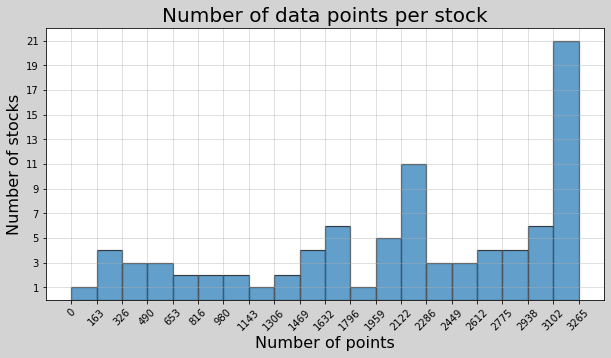
\includegraphics[width=0.7\textwidth]{figures/preprocessing/histogram_size.png}
    \caption{Histogram of the number of data points per stock.}
    \label{fig:histogram_size}
\end{figure}

\begin{figure}[H]
    \centering
    \begin{minipage}[t]{0.75\textwidth}
        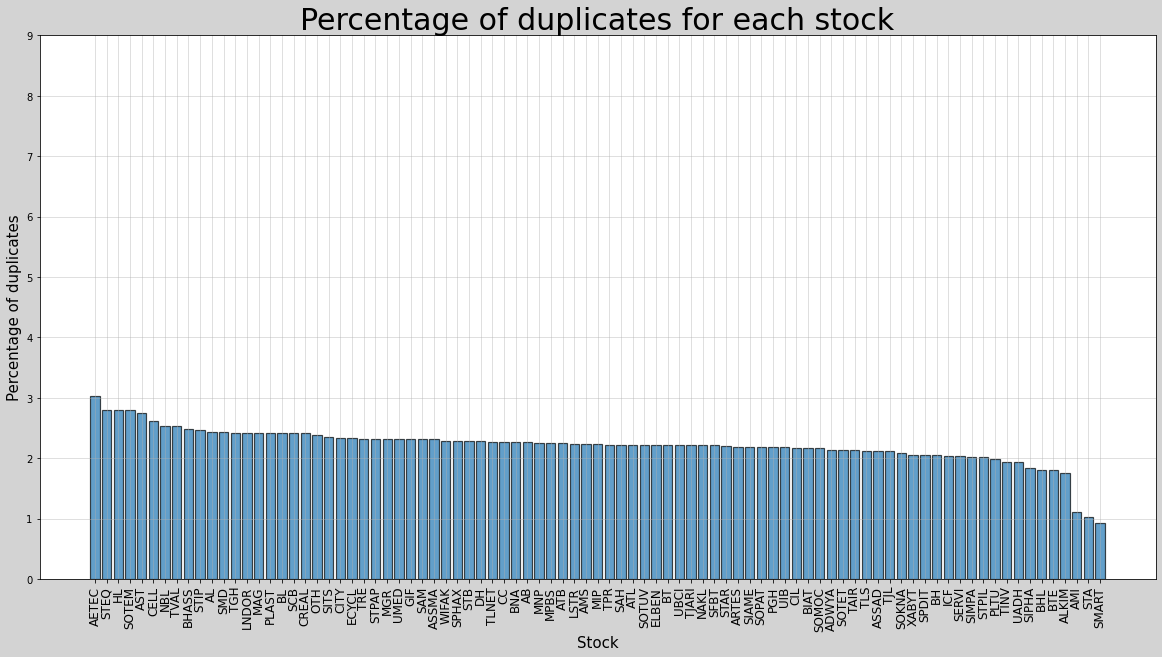
\includegraphics[width=\textwidth]{figures/preprocessing/bar_duplicates.png}
        \caption{Percentage of missing values per stock. The stocks are sorted by decreasing percentage of missing values.}
        \label{fig:bar_duplicates}
    \end{minipage}
\end{figure}

\begin{figure}[H]
    \centering
    \begin{minipage}[t]{0.75\textwidth}
        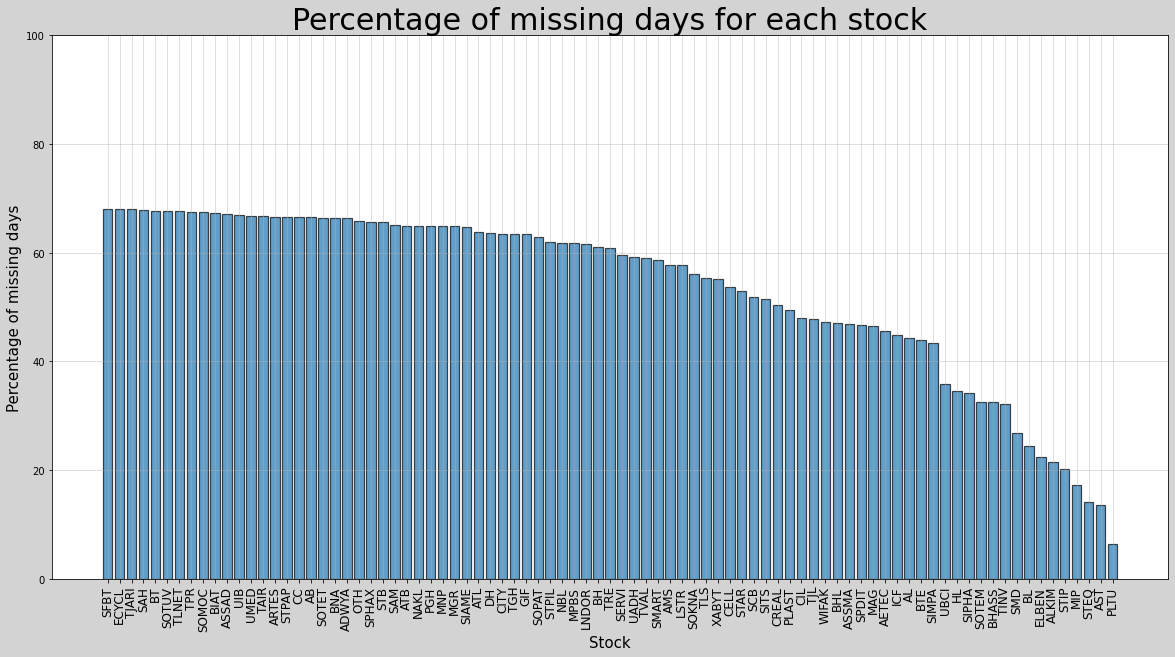
\includegraphics[width=\textwidth]{figures/preprocessing/bar_missing_days.png}
        \caption{Percentage of missing days per stock. The stocks are sorted by decreasing percentage of missing days.}
        \label{fig:bar_missing_days}
    \end{minipage}
\end{figure}

\begin{figure}[H]
    \centering
    \begin{minipage}[t]{0.7\textwidth}
        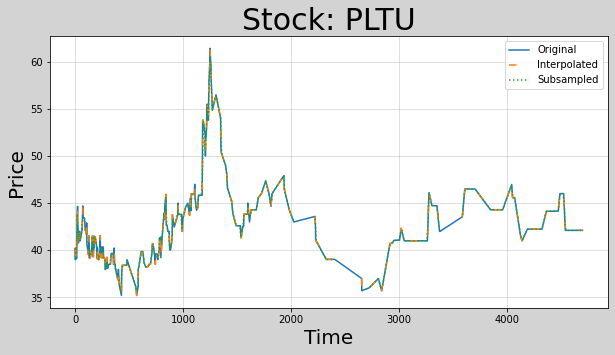
\includegraphics[width=\textwidth]{figures/preprocessing/subsample.png}
        \caption{Comparison of the original data and the sub-sampled data on the "Placement de Tunisie - Sicaf" (PLTU) stock.}
        \label{fig:subsample}
    \end{minipage}
\end{figure}

\subsection{Results figures}

\begin{figure}[H]
    \centering
    \begin{minipage}[t]{0.52\textwidth}
        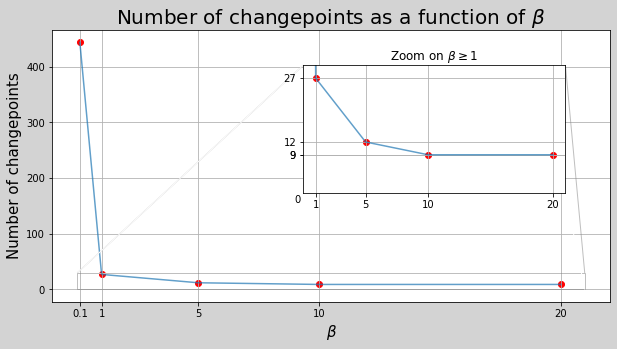
\includegraphics[width=\textwidth]{figures/results/cgpts_beta.png}
        \caption{Number of changepoints detected as a function of the penalty parameter $\beta$.}
        \label{fig:cgpts_beta}
    \end{minipage}
\end{figure}

\begin{figure}
    \centering
    \begin{minipage}[t]{0.42\textwidth}
        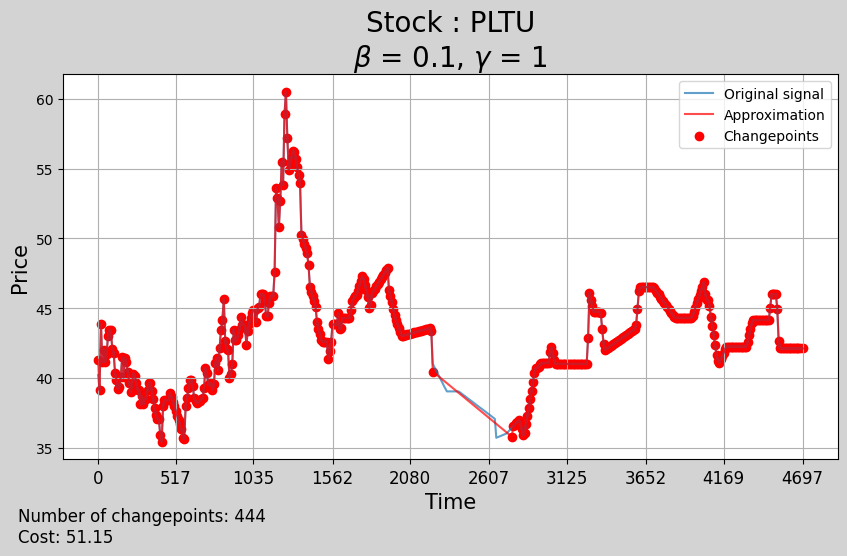
\includegraphics[width=\textwidth]{figures/results/beta_analysis_scale_1_stock_PLTU/beta_0.1.png}
    \end{minipage}
    \begin{minipage}[t]{0.42\textwidth}
        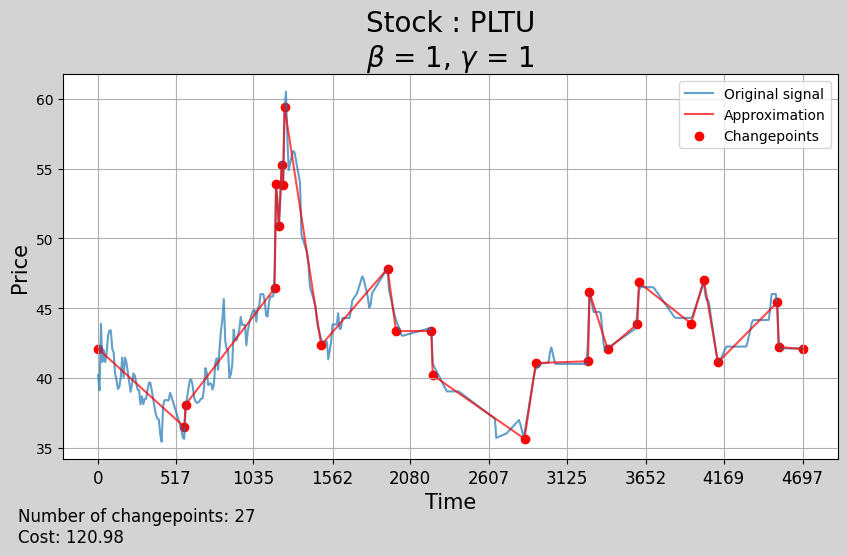
\includegraphics[width=\textwidth]{figures/results/beta_analysis_scale_1_stock_PLTU/beta_1.png}
    \end{minipage}

    \begin{minipage}[t]{0.42\textwidth}
        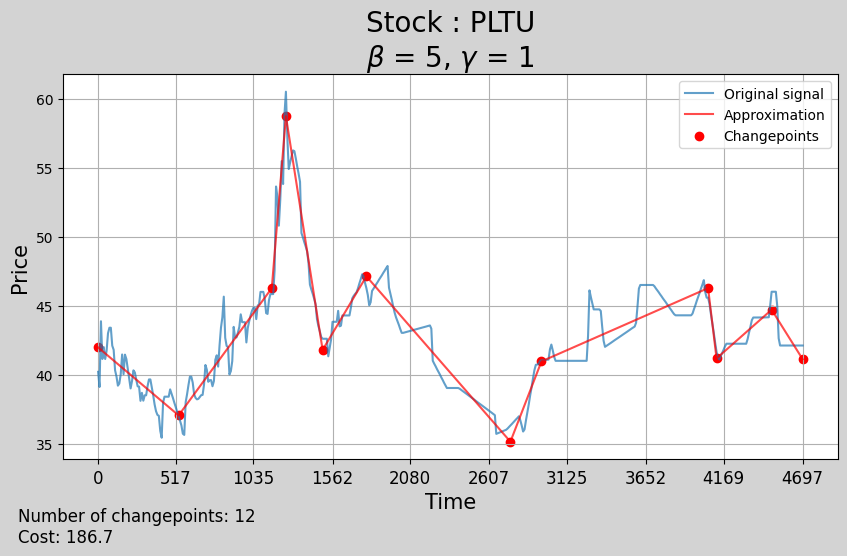
\includegraphics[width=\textwidth]{figures/results/beta_analysis_scale_1_stock_PLTU/beta_5.png}
    \end{minipage}
    \begin{minipage}[t]{0.42\textwidth}
        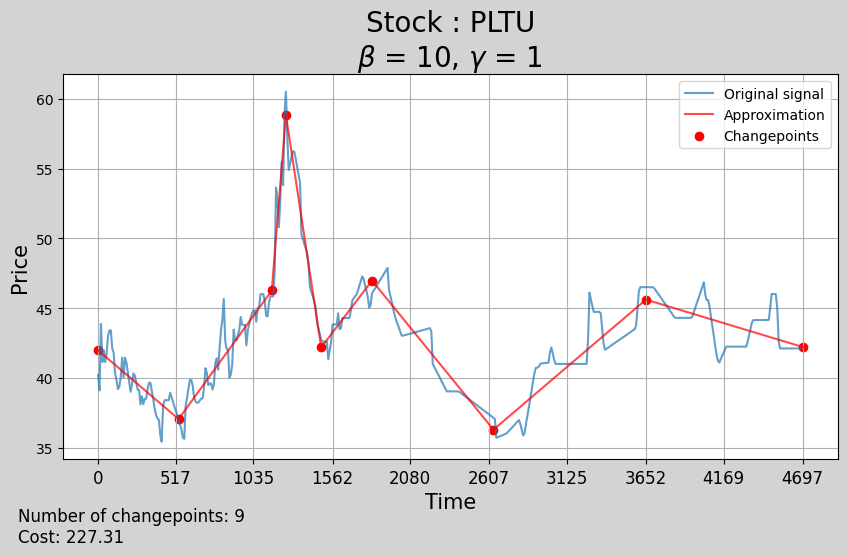
\includegraphics[width=\textwidth]{figures/results/beta_analysis_scale_1_stock_PLTU/beta_10.png}
    \end{minipage}

    \begin{minipage}[t]{0.42\textwidth}
        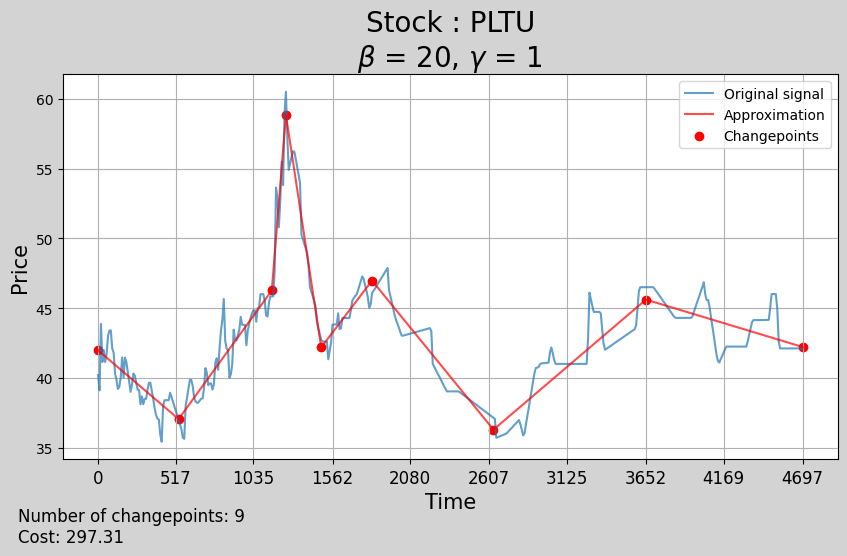
\includegraphics[width=\textwidth]{figures/results/beta_analysis_scale_1_stock_PLTU/beta_20.png}
    \end{minipage}
    \begin{minipage}[t]{0.42\textwidth}
        \hspace{0.42\textwidth}
    \end{minipage}
    \caption{Approximations obtained for values of $\beta \in \{0.1, 1, 5, 10, 20\}$ and $\gamma = 1$, on the "Placement de Tunisie - Sicaf" (PLTU) stock.}
    \label{fig:approximations_beta}
\end{figure}

\begin{figure}[H]
    \centering
    \begin{minipage}[t]{0.42\textwidth}
        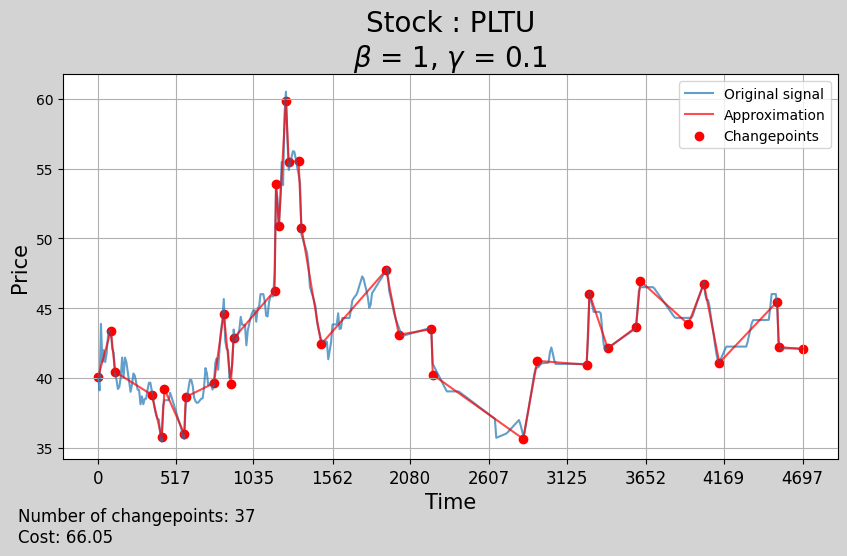
\includegraphics[width=\textwidth]{figures/results/scale_analysis_beta_1_stock_PLTU/scale_0.1.png}
    \end{minipage}
    \begin{minipage}[t]{0.42\textwidth}
        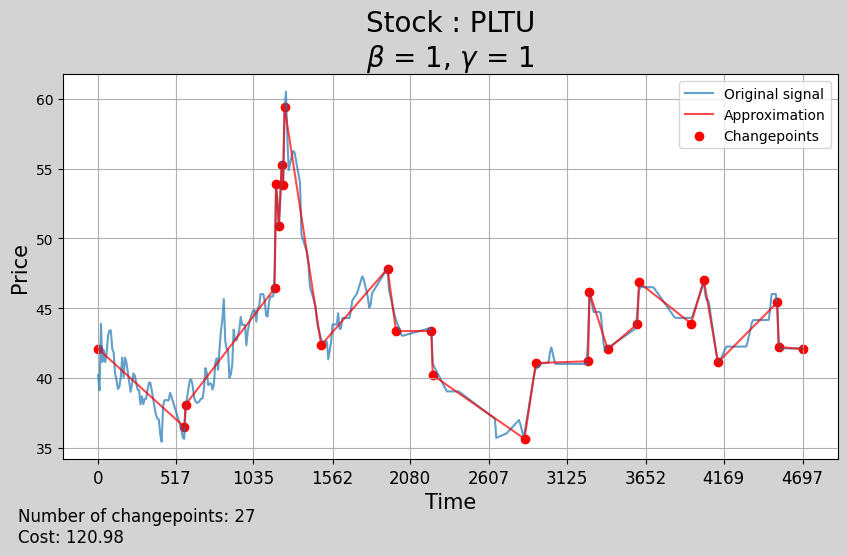
\includegraphics[width=\textwidth]{figures/results/scale_analysis_beta_1_stock_PLTU/scale_1.png}
    \end{minipage}

    \begin{minipage}[t]{0.42\textwidth}
        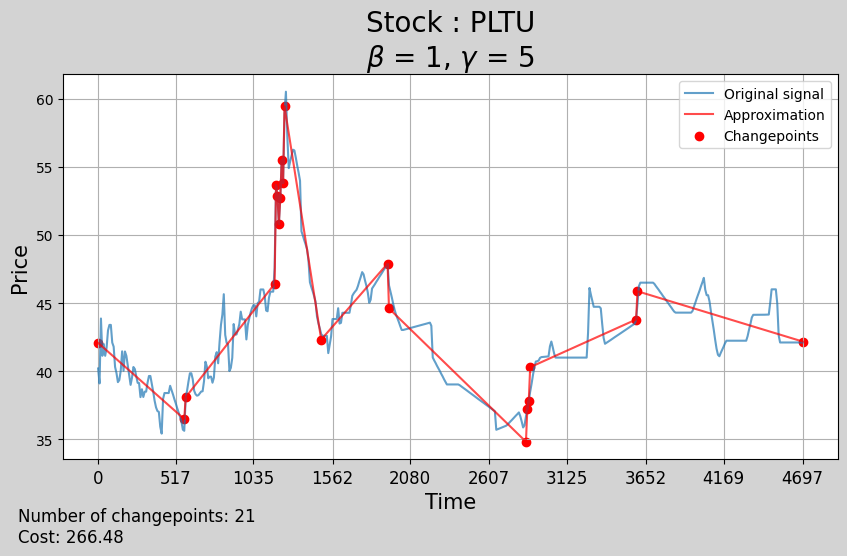
\includegraphics[width=\textwidth]{figures/results/scale_analysis_beta_1_stock_PLTU/scale_5.png}
    \end{minipage}
    \begin{minipage}[t]{0.42\textwidth}
        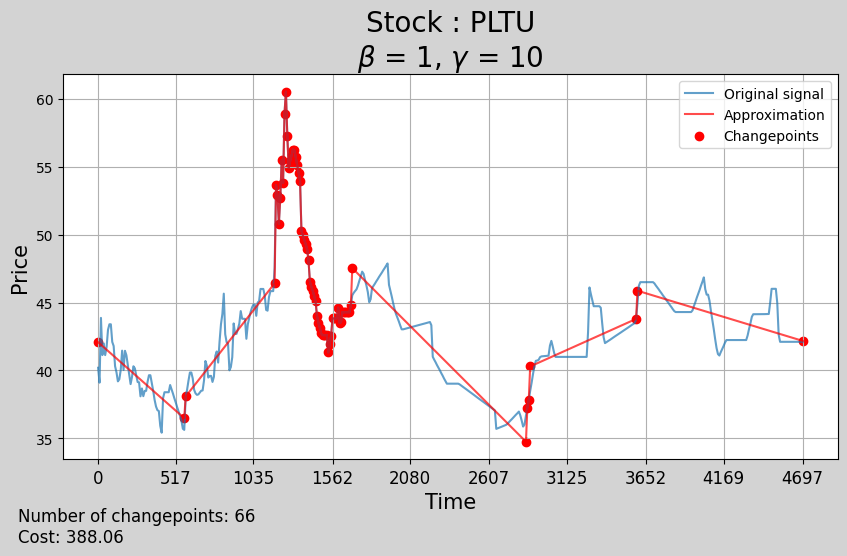
\includegraphics[width=\textwidth]{figures/results/scale_analysis_beta_1_stock_PLTU/scale_10.png}
    \end{minipage}

    \begin{minipage}[t]{0.42\textwidth}
        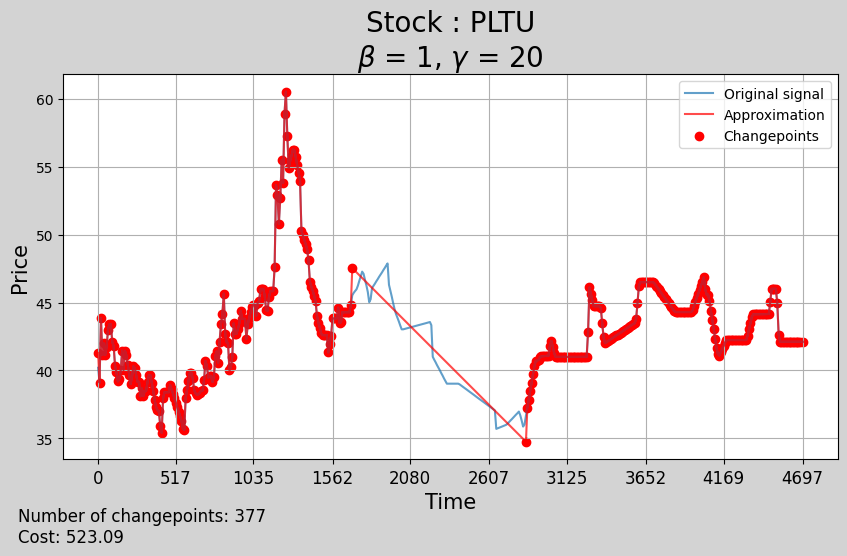
\includegraphics[width=\textwidth]{figures/results/scale_analysis_beta_1_stock_PLTU/scale_20.png}
    \end{minipage}
    \begin{minipage}[t]{0.42\textwidth}
        \hspace{0.42\textwidth}
    \end{minipage}

    \caption{Approximations obtained for values of $\gamma \in \{0.1, 1, 5, 10, 20\}$ and $\beta = 1$, on the "Placement de Tunisie - Sicaf" (PLTU) stock.}
    \label{fig:approximations_gamma}
\end{figure}

\end{document}
